\pagecolor{gray!10}%
Full Name: \hfill AP Calculus BC \\[22pt]
Date: \hfill Chapter 3 Practice Test \\[22pt]
\textbf{Multiple Choice Section} \hfill \textbf{20 Minutes; No Calculator} \\[11pt]

\begin{center}
    \textbf{Show All Work}
\end{center} \vspace{11pt}

\begin{questions}
    %Question 1
    \question $\int_1^8 \sqrt[3]{x^2} = $ \\

    \begin{oneparchoices}
        \choice $\dfrac{3}{5}$
        \choice $\dfrac{9}{2}$
        \choice $3$
        \choice $\dfrac{93}{5}$
        \choice $\dfrac{96}{5}$
    \end{oneparchoices} \par \horizontalline

    %Question 2
    \question $\int_1^8 \dfrac{1}{\left(2 + \sqrt[3]{x}\right)\sqrt[3]{x^2}} = $ \\

    \begin{oneparchoices}
        \choice $\dfrac{7}{2}$
        \choice $\dfrac{21}{2}$
        \choice $\dfrac{1}{3}\ln\dfrac{3}{2}$
        \choice $\ln\dfrac{3}{2}$
        \choice $3\ln\dfrac{4}{3}$
    \end{oneparchoices} \par \horizontalline

    %Question 3
    \question Based on the information below, find $\int_1^{-2} (3g(x) + 2f(x)) \,\mathrm{d}x$ \begin{align*}
        \arraycolsep=55pt\def\arraystretch{2.2} 
        \begin{array}[c]{|c|c|}
            \hline
            \int_{-2}^5 f(x) \,\mathrm{d}x = -2 & \int_1^5 f(x) \,\mathrm{d}x = 3 \\[5.5pt] \hline
            \int_{-2}^1 g(x) \,\mathrm{d}x = 4 & \int_5^1 g(x) \,\mathrm{d}x = 9 \\[5.5pt] 
            \hline
        \end{array}
    \end{align*}

    \begin{oneparchoices}
        \choice $-8$
        \choice $-2$
        \choice $0$
        \choice $3$
        \choice $5$
    \end{oneparchoices} \par \horizontalline

    \newpage

    %Question 4
    \question For $t \geq 0$ hours, $H$ is a differentiable function of $t$ that gives the rate of change in temperature, in degrees Celsius per hour, at an Arctic weather station. In what units would $\dfrac{1}{t}\int_0^t H'(x) \,\mathrm{d}x$ be measured? \\

    \begin{oneparchoices}
        \choice hours
        \choice degrees Celsius
        \choice degrees Celsius per hour \\[11pt]
        \makebox[0.07\textwidth] \choice degrees Celsius per hour per hour
        \makebox[0.20\textwidth] \choice hours per degrees Celsius
    \end{oneparchoices} \par \horizontalline

    %Question 5
    \question $\int_0^1 x^2\tan \left(x^3\right) \,\mathrm{d}x = $ \\

    \begin{oneparchoices}
        \choice $\dfrac{1}{3}\sec^2 (1)$
        \choice $\dfrac{1}{3}\sec^2 (1) - \dfrac{1}{3}$
        \choice $\dfrac{1}{3}\ln |\sec (1)| + \dfrac{1}{3}$ \\[11pt]
        \makebox[0.23\textwidth] \choice $\dfrac{1}{3}\ln |\sec (1)|$
        \makebox[0.26\textwidth] \choice $\dfrac{1}{3}\ln |\sec (3)|$
    \end{oneparchoices} \par \horizontalline

    %Question 6
    \question A ski resort uses a snow machine to control the snow level on a ski slope. Over a $24$-hour period the volume of snow added to the slope per hour is modeled by the equation $S(t)$. The rate that the snow melts is modeled by $M(t)$. Both $M(t)$ and $S(t)$ are measured in $\si{yd^3 \per h}$ and $t$ is measured in hours for $0 \leq t \leq 24$. At time $t = 0$, the slope holds $50 \si{yd^3}$ of snow. Which of the following expresses the average rate of change in the number of cubic yards of snow falling on the slope at $t$ hours? \\

    \begin{oneparchoices}
        \choice $\int_0^t S(x) \,\mathrm{d}x$
        \choice $\dfrac{1}{t}\int_0^t S(x) \,\mathrm{d}x$
        \choice $S(t)$ \\[11pt]
        \makebox[0.25\textwidth] \choice $S'(t)$
        \makebox[0.25\textwidth] \choice $\dfrac{\displaystyle\int_0^t S(x) \,\mathrm{d}x - 50}{t - 0}$
    \end{oneparchoices} \par \horizontalline

    \newpage

    %Question 7
    \question In the graph below, $A$, $B$, $C$, and $D$ are positive numbers that represent the areas between the curve $y = f(x)$ and the $x$-axis. If $A = 4$, $B = 8$, $C = 11$, and $D = 15$, what is the average value of $y = f(x)$ on $x \in [0, \, 8]$?
    \begin{center}
        
\includegraphics[width = 0.55\textwidth]{\graphicsdir Chapter 3 Graphics/PT-Graphic1.png}
    \end{center}

    \begin{oneparchoices}
        \choice $-1$
        \choice $1$
        \choice $8$
        \choice $8$
        \choice $48$
    \end{oneparchoices} \par \horizontalline

    %Question 8
    \question Find the average rate of change of $y = \cos (3x)$ on $x \in \left[0, \, \dfrac{\pi}{6}\right]$. \\
    
    \begin{oneparchoices}
        \choice $\dfrac{1}{3}$
        \choice $1$
        \choice $3$
        \choice $-\dfrac{6}{\pi}$
        \choice $\dfrac{2}{\pi}$
    \end{oneparchoices} \par \horizontalline

    %Question 9
    \begin{center}
        
\includegraphics[width = 0.5\textwidth]{\graphicsdir Chapter 3 Graphics/PT-Graphic2.png}
    \end{center}
    \question The approximate value of $\int_0^{10} f(x) \,\mathrm{d}x$, using 5 right-hand rectangles with equal width, is \\

    \begin{oneparchoices}
        \choice $20$
        \choice $24$
        \choice $28$
        \choice $32$
        \choice $36$
    \end{oneparchoices} \par \horizontalline
\end{questions} 

\newpage
\stepcounter{sectioncount}

\textbf{Free Response Section} \hfill \textbf{35 Minutes; Calculator Allowed} \\[11pt]

\begin{center}
    \textbf{Show All Work}
\end{center}
\vspace{11pt}

\begin{questions}
    \question Consider the function $g(x) = x\cos \left(\dfrac{\pi x^2}{4}\right)$ which has the graph below. \begin{align*}
        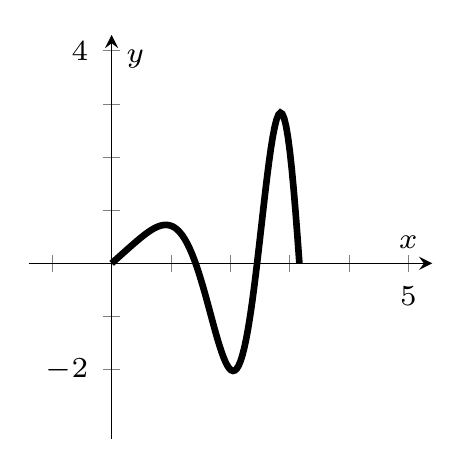
\begin{tikzpicture}[scale = 1.5]
            \begin{axis}[
                axis lines = middle,
                label style={font=\scriptsize},
                tick label style={font=\scriptsize},
                xlabel = $x$,
                ylabel = $y$,
                domain = 0:3.162,
                samples = 100,
                width=5cm,
                height=5cm,
                xmin = -1.4, xmax = 5.4,
                xtick = {-1, 0, 1, 2, 3, 4, 5},
                xticklabels = {, , , , , , $5$},
                ymin = -3.3, ymax = 4.3,
                ytick = {-2, -1, 0 , 1, 2, 3, 4},
                yticklabels = {$-2$, , , , , , $4$}
            ]
              \addplot[ultra thick] {x * cos(deg((pi * x * x) / 4))};
            \end{axis}
        \end{tikzpicture}
    \end{align*}
    Note that the zeroes are at $x = 0, \, \sqrt{2}, \, \sqrt{10}$. \\

    \begin{parts}
        \part Show the $u$-sub setup for $\int_0^{\sqrt{10}} g(x) \,\mathrm{d}x$ and solve it by calculator.

        \vfill

        \parthline

        \part Set up, but do not solve, an integral expression to determine the area between $y = g(x)$ and the $x$-axis on $x \in \left[0, \, \sqrt{10}\right]$. 

        \vfill
    \end{parts}

    \horizontalline

    \newpage

    \question \begin{center}
        \underline{The Carbon Sequestration Problem}
    \end{center}
    
    One innovative approach to global warming is to capture carbon dioxide that is created as a byproduct of producing concrete and storing the $\mathrm{CO_2}$ in the sandstone in depleted natural gas fields. At a particular site on a particular day, the $\mathrm{CO_2}$ is injected into the sandstone at a rate of \begin{align*}
        I(t) = 121\sin \left(\dfrac{\pi}{65}t^2\right).
    \end{align*}
    The $\mathrm{CO_2}$ stabilizes the ground and forces remaining natural gas upward where it can be extracted at a rate of \begin{align*}
        E(t) = 50 = 50\cos \left(\dfrac{\pi}{8}t\right).
    \end{align*}
    $I(t)$ and $E(t)$ are measured in metric tons per hour and $t$ is measured in hours where $0 \leq t \leq 8$. \\

    \begin{parts}
        \part How many metric tons of $\mathrm{CO_2}$ is injected into the field over $0 \leq t \leq 8$?

        \vspace{3.5cm}

        \parthline
        
        \part Find the value of $I(4)$ and $I'(4)$. Using the correct units, explain the meaning of both. 

        \vfill

        \parthline

        \newpage

        \part Find the time if any, when the rate of injection of $\mathrm{CO_2}$ is equal the rate of extraction of natural gas. 

        \vfill

        \parthline

        \part Find the total change of gasses in the sandstone during this 8-hour day. Using the correct units, explain the results.

        \vfill
    \end{parts}

    \horizontalline

    \newpage

    \question With $89.5$ sacks in his 14-year career, Bryant Young is the 49ers all-time sack leader. The table below shows the rate $Y(g)$, measured in sacks per game, during his four most productive seasons, 1996 to 1999. \begin{align*}
        \arraycolsep=16.5pt\def\arraystretch{1.5}
        \begin{array}{|c|c|c|c|c|c|}
            \hline
            g \text{ (games completed)} & 28 & 44 & 56 & 68 & 84 \\ \hline
            Y(g) \text{ (sacks per game)} & 0.5 & 0.72 & 0.33 & 0.79 & 0.69 \\
            \hline
        \end{array}
    \end{align*}

    \begin{parts}
       \part Using a right-hand Riemann approximation, determine the approximate number of sacks Bryant Young had during the four years. Round to the nearest whole number. 

        \vfill

        \parthline

        \part Using the data on the table, estimate $Y'(75)$. Based on this estimate and the data on the table, was Young's sack total increasing at an increasing or decreasing rate? Using the correct units, explain your answer.

        \vfill

        \parthline

        \newpage

        \begin{align*}
            \arraycolsep=16.5pt\def\arraystretch{1.5}
            \begin{array}{|c|c|c|c|c|c|}
                \hline
                g \text{ (games completed)} & 0 & 19 & 21 & 41 & 57 \\ \hline
                B(g) \text{ (sacks per game)} & 0 & 0.68 & 0.62 & 0.98 & 1.16 \\
                \hline
            \end{array}
        \end{align*}

        \part The table above shows Nick Bosa's sack rates over his first four seasons. Use a right-hand Riemann approximation to approximate $\dfrac{1}{50}\int_0^{50} B(g) \,\mathrm{d}g \forcespace$. Using the correct units, explain the result in the context of the problem.

        \vfill

        \parthline

        \part Disregarding his injury-shortened 2020 season, a model for Bosa's sack rate per game can be given with the equation \begin{align*}
            S_B(g) = 0.15\sqrt{g}.
        \end{align*}
        To the nearest whole number, how many more sacks than Bryant Young's does this model predict Nick Bosa will have between their 28th and 84th games?

        \vfill
    \end{parts}

    \horizontalline
\end{questions}

\newpage

\pagecolor{white}

